%==============================================================================
% intervals.tex
%==============================================================================

\chapter{Intervals}
\label{cha:intervals}

Intervals \cite{Matsakis2009b} are a new, higher-level primitive for
parallel programming with which programmers directly construct the
program schedule. They are under active development at ETH Zürich as
part of the PhD research of Nicholas Matsakis \cite{Matsakis2010}.

\section{Introduction}
\label{sec:intervals-introduction}

Existing primitives for synchronizing the control-flow of parallel
threads, such as signals and barriers, are low-level and dangerous to
use. They require careful attention to implementation details to
achieve good performance, and they are prone to errors, particularly
deadlocks and race conditions.

Intervals are a higher-level alternative that make parallel
programming safer while retaining the flexibility and efficiency of
threads. In the Intervals model, users create lightweight tasks and
order them using explicit \emph{happens before} relations
\cite{Lamport1978}. Users need not specify when a thread should block
or acquire a lock. Instead they specify when a task should execute
relative to other tasks, and what locks it should hold when it
executes. The details of making this schedule pass are left to the
runtime system.

The intervals API supports arbitrary \emph{happens before} relations
making the model very flexible. Intervals can be used to emulate
existing thread primitives \cite{Matsakis2009b}, but they can also be
used to easily create program schedules for which no standard thread
primitives exist, such as peer-to-peer synchronization.

One of the primary goals in developing intervals is that program
errors should not lead to deadlocks. This includes both misuse of the
APIs but also miscellaneous errors which causes tasks to abort
unexpectedly, such as dereferencing a null pointer
\cite{Matsakis2009}. A further goal is that an error in one task
should prevent other, dependent tasks from executing
\cite{Matsakis2010a}.

\section{Model}
\label{sec:intervals-model}

Intervals are first-class objects in the programming language that
represent the slice of program time used to execute a parallel
task. Intervals are structured hierarchically in a tree. The root of
the interval tree represents the entire program execution. Program
execution itself begins in a child of the root interval.

The conceptual model for intervals consists of points in time ordered
by a \emph{happens before} relation. In the model, an interval
\lstinline|i| consists of a pair of points -- \lstinline|i.start| and
\lstinline|i.end| -- called the start and end point. The start point
represents the moment when the interval begins execution. The end
point represents the moment when the interval's task is
completed. Programmers may introduce arbitrary ordering constraints by
adding \emph{happens before} edges between the start or end points of
different intervals. An edge \lstinline|p1 $\rightarrow$ p2| indicates
that the point \lstinline|p1| must occur before the point
\lstinline|p2|. It also indicates that any memory writes which
\emph{happen before} \lstinline|p1| must be visible to \lstinline|p2|.

An interval can be associated with one or more locks. The intervals
runtime will automatically acquire those locks before the interval's
start point occurs and release them after its end point has occurred.

When an interval executes, it begins by invoking the sequential method
\lstinline|run()|. \lstinline|run()| may either perform the task
directly or create a number of subintervals to achieve the task in
parallel. These subintervals begin to execute once the
\lstinline|run()| method has completed and they are ready to run. A
subinterval is ready to run when it could execute without violating
the \emph{happens before} relation. It will be executed when it is
ready and acquired all its locks.

\begin{figure}[htb]
  \centering
  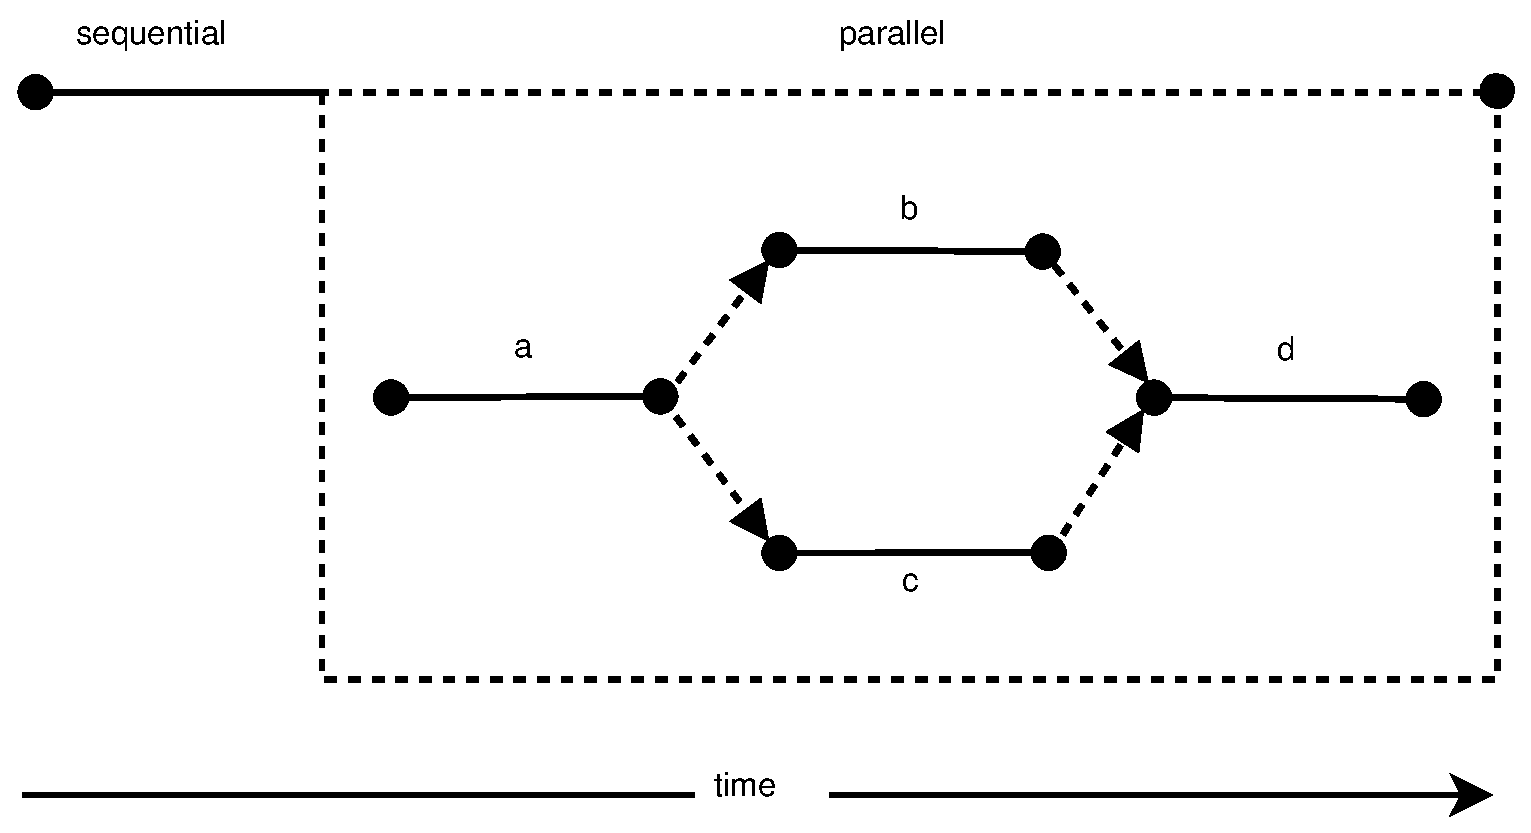
\includegraphics[width=0.96\textwidth]{intervals/interval-graph}
  \caption[Example interval graph]{Example interval graph: Showing an
    interval and its subintervals \lstinline|a|, \lstinline|b|,
    \lstinline|c| and \lstinline|d|.}
  \label{fig:interval-graph}
\end{figure}

The interval model can be depicted as a graph, as shown in Figure
\ref{fig:interval-graph}. The graph contains a single interval with
four subintervals, \lstinline|a|, \lstinline|b|, \lstinline|c| and
\lstinline|d|. The start and end points of each interval are
represented as opaque circles. The subintervals of an interval are
enclosed in a dashed box. This dashed box is omitted for leaf
intervals.

The dashed edges connecting different points indicate user-specified
additions to the \emph{happens before} relation. For example, the end
of \lstinline|a| \emph{happens before} the start of \lstinline|b| and
\lstinline|c| and the ends of \lstinline|b| and \lstinline|c| both
\emph{happen before} the start of \lstinline|d|.

\section{Java API}
\label{sec:intervals-java-api}

In the Java API, intervals are represented as instances of the
abstract class \lstinline|Interval| (Listing
\ref{lst:interval-class}). \lstinline|Interval| provides immutable
fields to access the interval's start point, end point, and parent,
along with an abstract \lstinline|run()| method which must be
redefined in a concrete subtype.

\begin{lstlisting}[
  style=Float, 
  caption={[\lstinline{Interval} class] \lstinline{Interval}: Serves as the base class for all intervals},
  label=lst:interval-class
]
public abstract class Interval {
  public final Interval parent;
  public final Point start;
  public final Point end;

  protected abstract void run();
}
\end{lstlisting}

Listing \ref{lst:interval-graph} contains Java code which uses the
Intervals API to construct the graph shown in figure
\ref{fig:interval-graph}.

\begin{lstlisting}[
  style=Float, 
  caption={[Intervals Java API example] Code to produce the sample interval graph shown in figure \ref{fig:interval-graph}},
  label=lst:interval-graph
]
public class ExampleInterval extends Interval {
  public ExampleInterval(Dependency dep, String name) {
    super(dep, name);
  }
  
  protected void run() {
    // Task
  }
  
  public static void main(String[] args) {
    Intervals.inline(new VoidInlineTask() { //*\label{lst:interval-graph-inline-start}
      public void run(Interval start) {
        Interval a = new ExampleInterval(start, "a"); //*\label{lst:interval-graph-new-start}
        Interval b = new ExampleInterval(start, "b");
        Interval c = new ExampleInterval(start, "c");
        Interval d = new ExampleInterval(start, "d"); //*\label{lst:interval-graph-new-end}
        
        Intervals.addHb(a, b); //*\label{lst:interval-graph-add-hb}
        Intervals.addHb(a, c);
        Intervals.addHb(b, d);
        Intervals.addHb(c, d);
        Intervals.schedule(); //*\label{lst:interval-graph-schedule}
      }
    }); //*\label{lst:interval-graph-inline-end}
  }
}
\end{lstlisting}

\subsection{Creating Intervals}
\label{sec:intervals-creating-intervals}

To start program execution, the programmer has to create a new child
of the root interval. One could for example use an inline interval to
do so. Inline intervals execute a task during the current interval and
do not return until the task has completed.

Lines \ref{lst:interval-graph-inline-start} --
\ref{lst:interval-graph-inline-end} create the inline subinterval
\lstinline|start| by providing an anonymous task class redefining its
\lstinline|run()| method. \lstinline|start| has four subintervals,
\lstinline|a|, \lstinline|b|, \lstinline|c| and \lstinline|d|. They
are created on lines \ref{lst:interval-graph-new-start} --
\ref{lst:interval-graph-new-end} and are normal, non-blocking
intervals.

\subsection{Scheduling Intervals}
\label{sec:intervals-scheduling-intervals}

Newly constructed intervals become eligible for execution once the
\lstinline|schedule()| method is invoked, as shown on line
\ref{lst:interval-graph-schedule} in Listing
\ref{lst:interval-graph}. This gives the user the opportunity to
construct any required dependencies or perform other
initialization. For example, adding the edge
\lstinline|a $\rightarrow$ b| on line \ref{lst:interval-graph-add-hb}
would be unsafe if \lstinline|b| could begin immediately, as it would
be possible that \lstinline|b.start| had already occurred before the
call to \lstinline|addHb()| could add the new dependency.

Explicit calls to \lstinline|schedule()| are unusual, however. This is
because the runtime automatically invokes \lstinline|schedule()| when
the \lstinline|run()| method of an interval returns.

%%% Local Variables: 
%%% mode: latex
%%% TeX-master: "thesis"
%%% End: